\documentclass[9pt]{beamer}
% \documentclass[notes, handout, 9pt]{beamer}
% \documentclass[handout, 9pt]{beamer}

\usepackage{import}
\subimport{../}{preamble.tex}
\subimport{../}{beamer-theme.tex}
\usepackage{svg}

% Location for all figures / pictures
\graphicspath{{pictures/}{figures/}}

% % Figures inline
\usepackage{tikz}
\usepackage{pgfplots}
\usetikzlibrary{calc}
\usetikzlibrary{shapes.multipart}
\usetikzlibrary{decorations.pathreplacing}
\usetikzlibrary{arrows.meta}
\usepgfplotslibrary{fillbetween}

\usepgfplotslibrary{ternary}

%--------------------------------------------------
% Presentation Information
%--------------------------------------------------
\title[Continuous Optimization]{Interior-Point Methods}
\author[]{\textbf{Bart Van Parys}}
\date{Fall 2026}
%--------------------------------------------------

\begin{document}

\begin{frame}  

  \maketitle

  \vspace{-2em}
  
    \begin{center}
    \begin{tabular}{lll}
      Instructor : & \textbf{Bart Van Parys} & \textbf{(\href{mailto:mastermath@vanparys.xyz}{mastermath@vanparys.xyz})} \\
    \end{tabular}
  \end{center}
  
\end{frame}

\begin{frame}{Previous Lectures}

  Unconstrained convex optimization :
  
  \[
    \min_{x\in\Re^n} \, f(x)
  \]

  \vfill
  
  \begin{itemize}
    \setlength\itemsep{1em}
  \item First-Order Methods : Slow global convergence
  \item Newton's Method : Fast local convergence
  \item Self-concordant functions make Newton method analysis affine invariant
  \item<2-> If $f\in \mc{SC}(2)$ is self-concordant, then
    \begin{itemize}
      \setlength\itemsep{0.5em}
    \item Dikin's ellipsoid in $\dom(f)$,
    \item damped Newton method converges globally,
    \item easy approximation of the quadratic convergence zone
      \[
        \norm{f'(x)}_{x,\star}\defn\sqrt{\iprod{f''(x)^{-1}f'(x)}{f'(x)}} \leq \frac{3-\sqrt{5}}{2}
      \]
    \end{itemize}
  \end{itemize}
  
\end{frame}

\section{Reflections on the Black-Box Model}

\begin{frame}{How to Prove Convexity ?}

  \begin{enumerate}
  \item Directly from the definition. \\
    Try this one :
    \[
      f : x \in \Re^n_{++} \mapsto \max \left\{\exp(\norm{x}^2_2), \lambda_{\max}(\textstyle\sum_{i=1}^n x_i A_i) - \log(x_1)\right\} + 5 x_n^4.
    \]
    \\[2em]
  \item<2-> \blue{By using the structure of the function}. By reducing the function via convexity preserving operations ($\max$, $\sum$) into convex elementary functions ($t\mapsto t^2$, $t\mapsto\exp(t)$, $t \mapsto -\log(t)$, \dots)
  \end{enumerate}
  
  \vfill

  \uncover<3->{
  \begin{tcolorbox}
    After all the effort, you pass this intricate structure to a black-box solver which \red{completely ignores} it!
  \end{tcolorbox}
  }
\end{frame}


\begin{frame}{Something Odd in Black-Box Methods for Convex Optimization}

  How do black-box methods approach a convex optimization problem ?

  \[
    \begin{array}{rl}
      \min_{x\in\Re^n} & f(x) \\[1em]
      \st & x\in Q
    \end{array}
  \]

  \vfill
  
  \begin{enumerate}
  \item Prove convexity of the objective function and constraints. \\
    Investigate a \emph{global} property of the optimization problem. \\[2em]

  \item<2-> Hide the problem in an opaque black-box which only gives you \emph{local} information.
    Typically $f(x)$, $f'(x)$, $f''(x)$, $\Pi_Q(x)$, \dots.
  \end{enumerate}
  
\end{frame}


\section{Barrier Formulations}

\begin{frame}{From Constrained to Unconstrained Optimization}

  Constrained optimization
  \[
    \begin{array}{rl}
      \min \set{f(  x)}{  x\in Q} \uncover<2->{= \min f(  x) + \red{\chi_Q(  x)},}
    \end{array}
  \]

  \begin{itemize}
  \item  Let $f : \Re^n\to\nRe$ be a twice differentiable convex function.\\
  \item  Let $Q \subseteq \Re^n$ be a closed convex set with {nonempty interior}.
  \item <2-> Let characteristic function $\chi_Q(  x) = 0$ if $  x\in Q$; $+\infty$ otherwise.

  \item<3-> Unconstrained objective $f(  x) + \chi_Q(  x)$ is \red{no longer twice differentiable}
  \item<3-> We can not apply Newton's method directly!
  \end{itemize}

  \vfill

  \uncover<4->{
  \textbf{Definition:} A barrier function for $Q$ is a function $F_Q : \Re^n\to\nRe$ which is
  \begin{itemize}
  \item Convex (preferably strictly) and lower semi-continuous
  \item Twice differentiable with $\dom(F_Q)=\blue{\interior}(Q)$
  \item This implies
    \[
      \lim_{x\to\bnd(Q)} \, F_Q(x)=+\infty.
    \]
  \end{itemize}
  }
\end{frame}

\begin{frame}{Self-Concordant Barriers?}

    \textbf{Example:}
  
    \begin{center}
    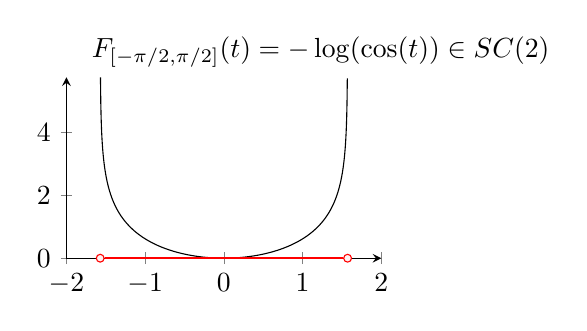
\begin{tikzpicture}
      
      \begin{axis}[
        %ticks=none,
        axis lines=left,
        y=0.4cm,            % y unit vector
        x=1cm,            % x unit vector
        clip=false,
        xmin =-2,
        xmax =2,
        %xlabel={ $\Re$},
        ylabel={ $F_{[-\pi/2, \pi/2]}(t)=-\log(\cos(t))\in \mc{SC}(2)$},
        x label style={at={(axis description cs:0.9,0.05)},anchor=west},
        y label style={at={(axis description cs:0.05,1)},rotate=-90,anchor=south west},
        ]
        
        \addplot[mark=none, black, samples=1000, domain=-2:2] {-ln(cos(deg(x)))};

        \node[circle, inner sep=1, draw=red, fill=red!5] (a) at (axis cs:-1.5707963267948966, 0) {};
        \node[circle, inner sep=1, draw=red, fill=red!5] (b) at (axis cs:1.5707963267948966, 0) {};
        \draw[draw=red, thick] (a) -- (b);
        
      \end{axis}
      
    \end{tikzpicture}
  \end{center}

  \vfill
  
  \textbf{Theorem:} Let $f\in SC(2)$ be a self-concordant function. Then for any point $\bar x\in \cl(\dom(f))$ and any sequence
  \(
    x_k\in\dom(f) \to \bar x
  \)
  we have that $f(x_k)\to +\infty$.

\end{frame}


\begin{frame}{From Constrained to Unconstrained Optimization}

  Transform unconstrained into constrained problem
  \[
    \begin{array}{rl}
      \min \set{f(x)}{x\in Q} = \min_{x} f(x) + \red{\chi_Q(x)},
    \end{array}
  \]

  \vfill

  Let $F_Q$ be a barrier function for the set $Q$.\\
  We approximate $f(x) + \red{\chi_Q(x)}$ by $f(x) + \blue{\mu F_Q(x)}$  for $\mu\downarrow 0$.

  \vfill
  
  \begin{center}
    \only<1-5>{
      \begin{tikzpicture}
        \begin{axis}[
          ticks=none,
          axis lines=left,
          y=0.5cm,            % y unit vector
          x=3cm,            % x unit vector
          ymax=5,
          xmin = -1.2,
          xmax = 1.2,
          % clip=true,
          title={$f(x)=-x$}
          ]

          \addplot +[mark=none, draw=blue, thick] table [x="X", y="F", col sep=comma] {data/barrier-function/f.csv};
          \draw[blue, thick, densely dotted] (axis cs:-1,-1) -- (axis cs:-1, 5);
          \draw[blue, thick, densely dotted] (axis cs:1,-1) -- (axis cs:1, 5);

          \only<2->{\addplot +[mark=none, draw=red] table [x="X", y="F", col sep=comma] {data/barrier-function/f_mu_3.0.csv};}
          \only<3->{\addplot +[mark=none, draw=red] table [x="X", y="F", col sep=comma] {data/barrier-function/f_mu_1.0.csv};}
          \only<4->{\addplot +[mark=none, draw=red] table [x="X", y="F", col sep=comma] {data/barrier-function/f_mu_0.3.csv};}
          \only<5->{\addplot +[mark=none, draw=red] table [x="X", y="F", col sep=comma] {data/barrier-function/f_mu_0.05.csv};}

          \node[above left] at (axis cs:-1,-1) {\small $-\frac{\pi}{2}$};
          \node[above right] at (axis cs:1,-1) {\small $\frac{\pi}{2}$};

        \end{axis}
        
      \end{tikzpicture}
    }
  \end{center}
  
\end{frame}

\begin{frame}{The Central Path}

  \vspace{-2em}
  \begin{center}
    \includesvg[width=0.4\textwidth]{central-path.svg}
  \end{center}
  \vspace{-2em}
  
  \vfill  
  
  Define the \emph{central path} $x(\mu)$ as 
  \[
    \begin{array}{rl}
      x^\star \in \arg\min\set{f(x)}{x \in Q} =& \arg \min \, f(x) +\chi_Q(x),\\[1em]
      x(\mu) = & \arg\min \, f(x) + \mu F_Q(x).
    \end{array}
  \]
  As $\dom(F_Q) = \interior(Q)$ we have that $x(\mu) \in \interior(Q)$.

\end{frame}

\begin{frame}{The Barrier Method for Approximating the Feasible Set}

  \textbf{Theorem :} If $F_Q( x)$ is bounded from below \red{and $f$ continuous}.  Then, \blue{$f( x(\mu)) \to f( x^\star)$} for $\mu \downarrow 0$.

  \vfill

  \uncover<2->{
  \textbf{Proof :} Let $m$ be the lower bound on the barrier function $F_Q$. Obviously, $ x(\mu)\in\interior(Q)$. We have
  \[
    \begin{aligned}
      \uncover<3->{\lim_{\mu \downarrow 0}} f( x(\mu)) + \mu (F_Q( x(\mu))-m) \leq &~\uncover<3->{\lim_{\mu \downarrow 0}} f(\bar{{x}}) + \mu (F_Q(\bar{{x}})-m) \uncover<4->{= f(\bar{{x}})} \quad \uncover<2->{\forall \bar{{x}} \in \interior(Q)}.\\
      \uncover<5->{\iff \lim_{\mu\downarrow 0} f( x(\mu)) + \mu (F_Q( x(\mu))-m) \leq &~\inf_{\bar{{x}}\in\interior(Q)} f(\bar{{x}})} \uncover<6->{ = f({x}^\star)}.\\
    \end{aligned}
  \]
  \uncover<7->{
    On the other hand
    \[
      f({x}^\star) \leq \uncover<8->{\lim_{\mu\downarrow 0}} f( x(\mu)) \leq \uncover<8->{\lim_{\mu\downarrow 0}} f( x(\mu)) + \mu (F_Q( x(\mu))-m).
    \]
  }
  \uncover<9->{Hence, $f( x^\star) \leq \lim_{\mu\downarrow 0} f( x(\mu)) \leq f( x^\star)$.}
  }
\end{frame}


\begin{frame}{General Strategy of Barrier Methods}

  \begin{algorithm}[H]
    \SetKwInput{Initialization}{Initialisation}
    \Initialization{Determine a point close to central path, say $\hat x(\mu_0) \approx x(\mu_0)$.}
    \For{$k\geq 1$}{
      Fix $\mu_{k+1} < \mu_k$. \\
      Starting from $\hat x(\mu_k)$, update to approximation $\hat x(\mu_{k+1})$ to $x(\mu_{k+1})$.
    }
    \caption{General Barrier Method}
  \end{algorithm}

  \vfill
  
  \textbf{Questions?}
  \begin{itemize}
  \item How to choose $F_Q$?
  \item How fast can we decrease $\mu$?
  \item How close must $\hat x(\mu_k)$ be to $x(\mu_k)$?
  \item How to efficiently compute $\hat x(\mu_{k+1})$ from $\hat x(\mu_{k})$?
  \item Stopping criteria?
  \end{itemize}
  
\end{frame}



\begin{frame}{General Strategy of Barrier Methods}

  \begin{algorithm}[H]
    \SetKwInput{Initialization}{Initialisation}
    \Initialization{Determine a point close to central path, say $\hat x(\mu_0) \approx x(\mu_0)$.}
    \For{$k\geq 1$}{
      Fix $\mu_{k+1} < \mu_k$. \\
      Starting from $\hat x(\mu_k)$, update to approximation $\hat x(\mu_{k+1})$ to $x(\mu_{k+1})$.
    }
    \caption{General Barrier Method}
  \end{algorithm}

  \vfill
  
  \textbf{Questions?}
  \begin{itemize}
  \item How to choose $F_Q$? \hfill \blue{Self-concordant function}
  \item How fast can we decrease $\mu$? \hfill \blue{Linearly :  $\mu_{k+1} \defn \tfrac{\mu_k}{(1+\delta)}$ }
  \item How close must $\hat x(\mu_k)$ be to $x(\mu_k)$? \hfill \blue{Quadratic convergence zone}
  \item How to efficiently compute $\hat x(\mu_{k+1})$ from $\hat x(\mu_{k})$? \hfill \blue{Newton's method}
  \item Stopping criteria? \hfill \blue{Duality}
  \end{itemize}
  
\end{frame}

\section{$\nu$-Self-concordant Barrier Functions}

\begin{frame}{Linear Optimization}

  Consider a convex problem with
  \[
    \begin{array}{rl}
      \min & f(x) \\
      \st    & x\in Q
    \end{array}
  \]
  and $f:\Re^n\to\Re$ a continuous function.\\

  \vfill

  \uncover<2->{
    Problem is equivalent to
    \[
      \begin{array}{rl}
        \min & z \\
        \st & (x, z) \in \epi(f) \defn \set{(x, z)}{f(x)\leq z} \\
             & x\in Q
      \end{array}
    \]
  }

\end{frame}

\begin{frame}{Moving on the Central Path and Staying Efficient}

  \begin{center}
    \begin{tcolorbox}[width=0.8\textwidth]
      \[
        \begin{array}{rl}
          \min_x \iprod{c}{x} + \chi_Q(x) & \to \min_x \iprod{c}{x} + \mu F_Q(x)\\[0.5em]
                                          & \to \min_x f(x; \mu) \defn \iprod{c}{x}/\mu +  F_Q(x)
        \end{array}
      \]
    \end{tcolorbox}
  \end{center}

  \vfill

  \textbf{Goal :} Reduce $\mu$ as fast as possible, while staying \blue{in the quadratic convergence zone}. 

  \begin{center}
    \includegraphics[height=4cm]{n-sc/n-sc.pdf}
  \end{center}
  
\end{frame}

\begin{frame}{Moving on the Central Path and Staying Efficient}

  \begin{center}
    \begin{tcolorbox}[width=0.7\textwidth]
      \[
        \min_x \iprod{c}{x} + \chi_Q(x) \to \min_x f(x; \mu)
      \]
    \end{tcolorbox}
  \end{center}

  \vfill

  \textbf{Goal :} Reduce $\mu$ as fast as possible, while staying \blue{in the quadratic convergence zone}. 

  \vfill
  Recall the Newton decrement
  \[
    \lambda^2(x; \mu) \defn \langle f''(x;\mu)^{-1} f'(x;\mu), f'(x; \mu) \rangle.
  \]
  We have that $\set{x}{\lambda(x; \mu)<\bar \lambda=\frac{3-\sqrt 5}{2}}$ is in the quadratic convergence zone.
  
\end{frame}

\begin{frame}{Self-Concordant Barriers}

  \textbf{Thought Experiment:}
  \begin{itemize}
  \item Assume for the moment that we are on the central path at $x(\mu)$. \\
    \begin{tcolorbox}
      For which $\mu_{-} \defn \frac{\mu}{1+\delta}$ is the point $x(\mu)$ in the quadratic convergence zone of $\min_x f(x, \red{\mu_{-}})$?
    \end{tcolorbox}

  \item<2-> Point $x(\mu)$ is in the quadratic convergence zone of $\min_x f(x; \red{\mu_{-}})$ if
    \begin{align*}
      \lambda(x(\mu); \mu_{-})^2 = & ~\langle f''(x(\mu); \mu_{-})^{-1} f'(x(\mu); \mu_{-}), f'(x(\mu); \mu_{-}) \rangle \leq \bar \lambda^2\\
      = & ~\delta^2 \langle F_Q''(x(\mu))^{-1} F'_Q(x(\mu)), F_Q'(x(\mu)) \rangle \leq \bar \lambda^2
    \end{align*}
    as $\frac{c}{\mu} + F'_Q(x(\mu))=0$ by the optimality of $x(\mu)$ and $f'(x(\mu); \mu_{-}) = -\delta F'_Q(x(\mu))$.
  \item<3->  Define a \emph{$\nu$-self-concordant barrier} $F_Q\in\mc{SC}(2)$ for $Q$ as 
    \[
      \exists \nu>0 : \langle F_Q''(x)^{-1} F'_Q(x), F_Q'(x)\rangle \leq \nu, \quad \forall x\in \interior(Q).
    \]
  \item<3->  With such barrier we can take $\delta^2 = \frac{\bar \lambda^2}{\nu}$. Ideally thus $\nu$ is as small as possible.
  \end{itemize}
  
\end{frame}

\begin{frame}{$\nu$-Self-Concordant Barrier Functions}

  A \emph{$\nu$-self-concordant barrier} $F:\Re^n\to\nRe$ is any function which satisfies
  \begin{itemize}
  \item $\forall x\in\dom(F)$, $h\in\Re^n$ : $\abs{F'''(x)[h, h, h]}\leq 2 \iprod{F''(x) h}{h}^{3/2}$,
  \item $\forall x\in \dom(F)$ : $\iprod{F''(x)^{-1} F'(x)}{F'(x)} \leq \nu$.
  \end{itemize}

  \vfill

  \begin{center}
    \begin{tabular}{llr}
      \hline
      $F$ & Domain & $\nu$\\
      \hline
      $t\mapsto-\log(t)$ & $\Re_{++}$ & 1\\
      $(x, t)\mapsto-\log(t^2-\norm{x}_2^2)$ & $L^n_{++}$ & 2\\
      $X\mapsto -\log(\det(X))$ & $S_{++}^n$ & n \\
      $t\mapsto-\log(\cos(t))$ & $(-\frac{\pi}{2},\frac{\pi}{2})$ & 1\\
      $(x, t)\mapsto-\log(\log(t)-x)-\log(t)$ & $\epi(\exp)$ & 2\\
      \hline
    \end{tabular}
  \end{center}

\end{frame}

% \begin{frame}{The Barrier for Semidefinite Optimization}

%   \textbf{Proof [$\star$]:} Let $F(X)\defn -\log(\det(X)) \in \mc{SC}(2)$ for $X\in S^n_{++}$. Let $X\in S^n_{++}$ and $H\in S^n$, then
%   \[
%     \iprod{F'(X)}{H}_F = \lim_{t\downarrow 0} \frac{-\log(\det(X+tH)/\det(X))}{t}=\lim_{t\downarrow 0} \frac{\log(\det(\mb I + t X^{-1/2} H X^{-1/2}))}{t}.
%   \]
%   Set $A\defn X^{-1/2} H X^{-1/2}$. We continue as
%   \[
%     \iprod{F'(X)}{H}_F = \lim_{t\downarrow 0} \sum_{i=1}^n\frac{\log(1+t\lambda_i(A))}{t}=-\sum_{i=1}^n {\lambda_i(A)}=-\rm{Tr}(A).
%   \]
%   Thus, $\iprod{F'(X)}{H}_F=-\iprod{I}{A}_F = -\iprod{X^{-1}}{H}_F$ and $F'(X)=-X^{-1}$. 
%   Observe that $(X+tH)(X^{-1}+t X^{-1} H X^{-1})=\mb I + \mc O(t^2)$, thus
%   \[
%     F''(X) H = \lim_{t\downarrow 0} \frac{-(X+tH)^{-1}+X^{-1}}{t} = \lim_{t\downarrow 0}\frac{-X^{-1}+t X^{-1} H X^{-1} + X^{-1}}{t} = X^{-1} H X^{-1},
%   \]
%   Thus, $F''(X)^{-1} H = X H X$ yielding $\iprod{F''(X)^{-1} F'(X)}{F'(X)}_F = n$. $F$ is a $n$-self-concordant barrier for $S^n_{+}$.
% \end{frame}

\begin{frame}{Building Self-Concordant Barriers}

  Let $f\in \mc{SCB}(\nu, Q)$ if $f$ is a $\nu$-self-concordant barrier for $Q$.

  \vfill
  
  \begin{itemize}
    \setlength\itemsep{1.5em}
  \item Let $f \in \mc{SCB}(\nu_f; Q_f)$ and $g \in \mc{SCB}(\nu_g; Q_g)$. \\
    Then, $f(x) + g(x) \in \mc{SCB}(\nu_f+\nu_g;Q_f\cap Q_g)$.
  \item Let $f \in \mc{SCB}(\nu_f; Q_f)$ and $g \in \mc{SCB}(\nu_g; Q_g)$. \\
    Then, $f(x) + g(y) \in \mc{SCB}(\nu_f+\nu_g;Q_f\times Q_g)$.
  \item<2-> Suppose that $K$ is a pointed closed convex cone with nonempty interior. \\
    Let $F\in\mc{SCB}(\nu, K)$ be \blue{logarithmically homogeneous}
    \[
      F(t x) = F(x) - \nu \log(t) \quad \forall t>0, ~x\in \interior(K).
    \]
    Then, $F^\star \in \mc{SCB}(\nu, -K^\star)$.
  \end{itemize}
  
\end{frame}

\begin{frame}{Example}

  \textbf{Example:}
  \[
    \begin{array}{rl}
      \min_{x\in \Re^n} & \norm{x}+ \lambda_{\max}(\textstyle\sum_{i=1}^n x_i A_i)
    \end{array}
  \]

  \begin{itemize}
  \item We can use the calculus of convex functions to prove that this is a convex problem.
  \item<2-> This calculus allows us to claim equivalence with the standard conic problem
    \[
      \begin{array}{rl}
        \min_{x, s, U} & s_1 + s_2 \\[0.5em]
        \st  & U = \textstyle s_2 I_n-\sum_{i=1}^n x_i A_i\\[0.5em]
                       & (x, s_1) \in L^n_{+}, \\[0.5em]
                       & U \in S^n_+
      \end{array}
    \]
  \item<3-> Please recall that equality constraints are of no concern to the Newton method.
  \item<4-> This calculus also leads us to use the $\nu=n+2$-self-concordant barrier function $F_Q(x, s, t) = -\log(s_1^2-\norm{x}^2)-\log(\det(U))$.
  \item<5-> Not really the best possible choice\dots
  \end{itemize}
  
\end{frame}

\begin{frame}{The Universal Barrier Function}


  \textbf{Definition:} We define the universal barrier of a set $Q$ as the function
  \[
    F^\star_Q(x) \defn \log({\rm{vol}}(Q^\circ(x)))
  \]
  where $Q^\circ(x)=\set{y\in\Re^n}{\iprod{y}{z-x}\leq 1 ~~\forall z\in Q}$.

  \vfill

  \textbf{Theorem:} For all $n\geq 1$, $F^\star_Q$ is an $n$-self-concordant barrier function for $Q$.

  \vfill

  \textbf{Remark:} this barrier function is not easy to compute.
  
\end{frame}

\section{Why are $\nu$-Self-Concordant Barriers so Good?}

\begin{frame}{A Half-Space Containing the Domain}

  \textbf{Theorem :} Let $F\in \mc{SCB}(\nu; Q)$. For every $x$ and $y$ in $Q$ we have $\iprod{F'(x)}{y-x}< \nu$.

  \vfill   

  \begin{center}
    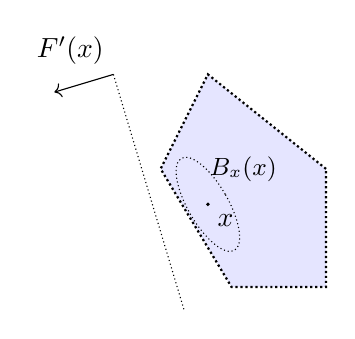
\begin{tikzpicture}[
      scale=1.5,
      % every node/.style={scale=1.5},
      ]

      \fill[draw=black, densely dotted, fill=blue!10, thick] (-1, 0) -- (-2, 0.8) -- (-2.4, 0) -- (-1.8, -1) -- (-1, -1) -- cycle;
      
      \node[black, inner sep=0.5, fill, circle] (x0) at (-2, -.3) {};
      \draw[black, rotate around={30:(x0)}, densely dotted] (x0) ellipse ({0.17} and {0.45});
      \node[below right, black] at (x0) {${x}$};
      \node at (-1.7, 0) {\gray{\small $B_x(x)$}};

      \uncover<2->{      
      \draw[densely dotted] (-2.8, 0.8) -- (-2.2, -1.2) ;
      \draw[->] (-2.8, 0.8) --+ (-0.5, -0.15);
      \node[above left] at (-2.8, 0.8) {$F'(x)$}; 
      }
    \end{tikzpicture}
  \end{center}


\end{frame}

\begin{frame}{Proof [$\star$]}

  \textbf{Proof [$\star$]:} Observe that for all $x\in \interior(Q)$ and $h\in \Re^n$:
  \[
    F \in \mc{SCB}(\nu, Q) \implies \sup_\lambda \, 2\iprod{F'(x)}{\lambda h} - \iprod{F''(x) \lambda h}{\lambda h} \leq \nu,
  \]
  or $\blue{\iprod{F'(x)}{h}^2 \leq \nu \iprod{F''(x)h}{h}}$ by optimizing over $\lambda$. We fix $x, y \in \interior(Q)$. Let $\phi(t) = \iprod{F'(x + t(y-x))}{y-x}$ for $t\in[0, 1]$. If $\phi(0)\leq 0$, there is nothing to prove. Suppose that $\phi(0) > 0$. Since $F\in \mc{SCB}(\nu;Q)$, we have $\phi(t)^2\leq \nu \phi'(t)$, therefore $\phi(t)>0$ for $t\in[0, 1]$ and
  \[
    \frac{1}{\nu} \leq \frac{\phi'(t)}{\phi(t)^2} = \left(-\frac{1}{\phi(t)}\right)' \implies \frac{t}{\nu} \leq \frac{1}{\phi(0)}-\frac{1}{\phi(t)}<\frac{1}{\phi(0)}.
  \]
  Thus, $\phi(0) = \iprod{F'(x)}{y-x} < \frac{\nu}{t}$ for $t\in [0, 1]$.

\end{frame}

\begin{frame}{Exact Algorithm Converges Linearly to Solution}

  \begin{center}
    \begin{tcolorbox}[width=0.7\textwidth]
      \[
        \min_x ~\iprod{c}{x} + \chi_Q(x) \to \min_{x} ~f(x; \mu)\defn \frac{\iprod{c}{x}}{\mu} + F_Q(x)
      \]
    \end{tcolorbox}
  \end{center}

  \vfill

  \begin{itemize}
    \setlength\itemsep{1em}
  \item We have already shown that $\lim_{\mu\downarrow 0}\iprod{c}{x(\mu)} = \iprod{c}{x^\star}$. \\ What about the \emph{speed of convergence}?
    
  \item<2-> Recall that $c+\mu F'_Q(x(\mu))=0$. We have
    \[
      \iprod{c}{x(\mu)}-\iprod{c}{x^\star} = -\mu \iprod{F'_Q(x(\mu))}{x(\mu)-x^\star}\leq \mu \nu.
    \]
  \item<2-> The convergence speed must hence be \emph{linear}.
  \end{itemize}
\end{frame}

\begin{frame}{Approximate Points to the Central Path are Good Enough}

  \textbf{Definition:} A point $x$ is centered in $\min_{x}f(x;\mu)$ if its Newton decrement is bounded by
  \[
     \norm{f'(x; \mu)}_{x, \star} = \norm{c/\mu+F'_Q(x)}_{x, \star} \leq\beta<1.
  \]

  \vfill
  
  \begin{center}
      \begin{tikzpicture}[scale=0.7,]
      \begin{ternaryaxis}[
        ticks=none,
        clip=false
        ]

        \addplot3[forget plot, fill=blue!10, opacity=1, draw=blue] 
        coordinates 
        {
          (1,0,0) 
          (0,1,0) 
          (0,0,1)
        }--cycle;
                
        \node (x0) at (axis cs:1/3,1/3,1/3) {};
        %\draw[draw=green, fill=green!20, thick] (x0) circle [radius=0.20];
        \draw[draw=orange, fill=orange!20, thick] (x0) circle [radius=0.06];
        \node[above right] at (x0){$ x(\mu)$};
        \node[fill=red,inner sep=0.7pt,circle] at (x0) {};

        % \only<2->{
        % \node (x1) at (axis cs:0.23121786065046332,0.30793757600101007,0.4608445614627931) {};
        % \draw[draw=green, fill=green!20, thick, opacity=0.5] (x1) circle [radius=0.18];
        % %\draw[draw=orange, fill=orange!20, thick] (x1) circle [radius=0.04];
        % \node[above right] at (x1){$\bold x(\mu_{k+1})$};
        % \node[fill=red,inner sep=0.7pt,circle] at (x1) {};
        % }

        \node[fill=red,inner sep=1pt,circle] (xa0) at (axis cs:0.32,0.36,0.32) {};
        \node[below left] at (xa0) {$ x$};
        
        \addplot3  [draw=red, thick] table [x="p1",y="p2", z="p3", col sep=comma] {data/path.csv}; 
        

        \node[fill=red,inner sep=0.7pt,circle] (xstar) at (axis cs:0,0,1) {};
        \node[right] at (xstar) {$ x^\star$};


      \end{ternaryaxis}
    \end{tikzpicture}

  \end{center}

  
  \textbf{Theorem :} Assume that $x$ is \emph{centered}, that is $\norm{c/\mu+F'_Q(x)}_{x, \star} \leq\beta$. Then,
  \[
    \iprod{c}{x} - \iprod{c}{x^\star} \leq \red{\mu}\left(\nu+\frac{\beta(\beta +\sqrt{\nu})}{1-\beta}\right).
  \]

\end{frame}

\begin{frame}{Proof [$\star$]}

  \textbf{Proof [$\star$] :} We know that $\iprod{c}{x(\mu)} - \iprod{c}{x^\star} \leq \mu \nu$. The missing part is
  \begin{align*}
    \iprod{c}{x} - \iprod{c}{x(\mu)} & = \mu \iprod{f'(x;\mu)- F'_Q(x)}{x-x(\mu)}\\
                                           & \leq \mu \left(\norm{f'(x;\mu)}_{x,\star}+\norm{F'_Q(x)}_{x,\star}\right)\norm{x-x(\mu)}_{x}.
  \end{align*}
  First, $\norm{f'(x;\mu)}_{x,\star} = \norm{c/\mu+ F'_Q(x)}_{x,\star}\leq \beta$. Also, $\norm{F'_Q(x)}_{x, \star}\leq \sqrt{\nu}$. Finally, we have shown in the self-concordant functions lecture that $\norm{x-x(\mu)}_x\leq \frac{\beta}{1-\beta}$.
  
\end{frame}


\begin{frame}{One Newton Step is Enough}

  \begin{center}

    \begin{tikzpicture}[
      scale=0.7,]
      
      \begin{ternaryaxis}[
        ticks=none,
        clip=false
        ]

        \addplot3[forget plot, fill=blue!10, opacity=1, draw=blue] 
        coordinates 
        {
          (1,0,0) 
          (0,1,0) 
          (0,0,1)
        }--cycle;
        

        \node (x1) at (axis cs:0.23121786065046332,0.30793757600101007,0.4608445614627931) {};
        %\draw[draw=green, fill=green!20, thick] (x1) circle [radius=0.18];
        \draw[draw=orange, fill=orange!20, thick] (x1) circle [radius=0.04];
        \node[above right] at (x1){$ x(\mu_-)$};
        \node[fill=red,inner sep=0.7pt,circle] at (x1) {};
        
        
        \node (x0) at (axis cs:1/3,1/3,1/3) {};
        % \draw[draw=green, fill=green!20, thick] (x0) circle [radius=0.20];
        \draw[draw=orange, fill=orange!20, thick] (x0) circle [radius=0.06];
        \node[above right] at (x0){$ x(\mu)$};
        \node[fill=red,inner sep=0.7pt,circle] at (x0) {};
        

        \node[fill=red,inner sep=1pt,circle] (xa0) at (axis cs:0.32,0.36,0.32) {};
        \node[below left] at (xa0) {$x$};

        

        
        \addplot3  [draw=red, thick] table [x="p1",y="p2", z="p3", col sep=comma] {data/path.csv}; 
        

        \node[fill=red,inner sep=0.7pt,circle] (xstar) at (axis cs:0,0,1) {};
        \node[right] at (xstar) {$ x^\star$};

        

        \node[fill=red,inner sep=1pt,circle] (xa1) at (axis cs:0.22121786065046332,0.32793757600101007,0.4508445614627931) {};
        \node[below] at (xa1) {$ x_-$};
        
        \draw[thick, ->] (xa0) -- (xa1);
      \end{ternaryaxis}
    \end{tikzpicture}

  \end{center}


  \textbf{Theorem :}
  Let $\beta < \frac{3-\sqrt{5}}{2}$ and $0<\delta \leq \frac{\sqrt{\beta}-\beta-\beta\sqrt{\beta}}{(\beta + \sqrt{\nu})(\sqrt{\beta}+1)}$.
  Do one Newton iteration
  \[
    \mu_{-} \defn \frac{\mu}{1+\delta}, \quad x_{-} \defn x - F''_Q(x)^{-1}\left(c/\mu_{-}+F'_Q(x)\right).
  \]
  on the problem $\min_x f(x; \mu_-)$.
  Then,
  \[
    \lambda \defn \norm{\frac{c}{\mu} + F'_Q(x)}_{x, \star}\leq \beta \implies \lambda_{-} \defn \norm{\frac{c}{\blue{\mu_{-}}} + F'_Q(\blue{x_{-}})}_{\blue{x_{-}}, \star}\leq \beta.
  \]

  \uncover<2->{
  \textbf{Remark:}
  \begin{itemize}
  \item We can take for instance $\beta\defn\frac{1}{10}$ and $\delta \defn\frac{1.4}{1+10\sqrt{\nu}}$.
  \end{itemize}
  }
\end{frame}

\begin{frame}{Proof [$\star$]}

    \begin{center}

    \begin{tikzpicture}[
      scale=0.7,]
      
      \begin{ternaryaxis}[
        ticks=none,
        clip=false
        ]

        \addplot3[forget plot, fill=blue!10, opacity=1, draw=blue] 
        coordinates 
        {
          (1,0,0) 
          (0,1,0) 
          (0,0,1)
        }--cycle;
        

        \node (x1) at (axis cs:0.23121786065046332,0.30793757600101007,0.4608445614627931) {};
        \draw[draw=green, fill=green!20, thick] (x1) circle [radius=0.18];
        \draw[draw=orange, fill=orange!20, thick] (x1) circle [radius=0.04];
        \node[above right] at (x1){$ x(\mu_{-})$};
        \node[fill=red,inner sep=0.7pt,circle] at (x1) {};
        
        
        \node (x0) at (axis cs:1/3,1/3,1/3) {};
        % \draw[draw=green, fill=green!20, thick] (x0) circle [radius=0.20];
        \draw[draw=orange, fill=orange!20, thick] (x0) circle [radius=0.06];
        \node[above right] at (x0){$ x(\mu)$};
        \node[fill=red,inner sep=0.7pt,circle] at (x0) {};
        

        \node[fill=red,inner sep=1pt,circle] (xa0) at (axis cs:0.32,0.36,0.32) {};
        \node[below left] at (xa0) {$ x$};

        

        
        \addplot3  [draw=red, thick] table [x="p1",y="p2", z="p3", col sep=comma] {data/path.csv}; 
        

        \node[fill=red,inner sep=0.7pt,circle] (xstar) at (axis cs:0,0,1) {};
        \node[right] at (xstar) {$ x^\star$};

        

        \node[fill=red,inner sep=1pt,circle] (xa1) at (axis cs:0.22121786065046332,0.32793757600101007,0.4508445614627931) {};
        \node[below] at (xa1) {$ x_{-}$};
        
        \draw[thick, ->] (xa0) -- (xa1);
      \end{ternaryaxis}
    \end{tikzpicture}

  \end{center}
  
  \textbf{Proof [$\star$]:} Let $\hat \lambda \defn \norm{c/\mu_{-} + F'_Q(x)}_{x, \star}$. Then $\hat \lambda \leq \lambda + \delta \norm{c}_{x, \star}/\mu$. Note
  \[
    \norm{c}_{x,\star}= \mu \norm{ f'(x; \mu)-F'_Q(x)}_{x, \star} \leq \mu(\lambda +\norm{F_Q'(x)}_{x,\star}) \leq \mu(\beta + \sqrt{\nu}).
  \]
  Since, $\iprod{c}{x}/\mu + F_Q(x) \in \mc{SC}(2)$, we have $\lambda_{-} \leq \frac{\hat \lambda^2}{(1-\hat \lambda)^2} \leq \left(\frac{\lambda+\delta(\beta + \sqrt{\nu})}{1-\lambda -\delta(\beta+\sqrt{\nu}) }\right)^2$ as $\hat \lambda \leq \sqrt{\beta}/(\sqrt\beta+1)<1$. One can show that $\lambda_-$ is smaller than $\beta$ for our particular choice of $\delta$.

  
\end{frame}

\section{Complexity}

\begin{frame}{The Final Algorithm}

    \begin{algorithm}[H]
      Find a barrier $F_Q\in \mc{SCB}(\nu; Q)$.\\
      Set $\beta\defn \tfrac{1}{10}$ and $\delta \defn \tfrac{1.4}{(1+10\sqrt{\nu})}$.\\
      \red{Determine a centered point $x_0$ such that $\norm{c/\mu_0+F'(x_0)}_{x_0, \star}\leq \beta$}\\
      \For{$k\geq 1$}{
      $\mu_{k+1} \defn \tfrac{\mu_k}{(1+\delta)}$. \\
      Perform Newton step :
      \[
        x_{k+1} = x_k - F''_Q(x_k)^{-1}\left(\tfrac{c}{\mu_{k+1}} +F_Q'(x_k) \right)
      \]
    }
    \caption{Self-Concordant Barrier Method}
  \end{algorithm}

  \vfill
  We have the optimality inequality:
  \[
    \iprod{c}{x_k} - \iprod{c}{x^\star} \leq \red{\frac{\mu_0}{(1+\delta)^k}}\left(\nu+\frac{\beta(\beta +\sqrt{\nu})}{(1-\beta)}\right) = \red{\frac{\mu_0}{(1+\delta)^k}}\left(\nu+\frac{\sqrt{\nu}}{9} + \frac{1}{90}\right).
  \]

  
\end{frame}

\begin{frame}{Example: Linear Optimization}

  Linear optimization problem
  \[
    \begin{array}{rl}
      \min_{x\in \Re^3} & x_1+2x_2+3x_3\\[0.5em]
      \st & x_1,~x_2, ~x_3\geq 0,\\[0.5em]
                        & x_1+x_2+x_3 = 1.
    \end{array}
  \]
  \textbf{Remarks:}
  \begin{itemize}
  \item Optimal solution $x = (1, 0, 0)$.
  \end{itemize}
  
  \vfill
 
  Transformation $x = (p_1, p_2, 1-p_1-p_2)$. \emph{Equivalent} problem
  \[
    \begin{array}{rl}
      \min_{x\in \Re^3} & -2p_1-1p_2+3\\[0.5em]
      \st & p_1\geq 0, ~p_2\geq 0, ~1-p_1-p_2\geq 0.
    \end{array}
  \]  
  with $p^\star = (1, 0)$.
\end{frame}

\begin{frame}{Example : Self-Concordant Barrier}

  The function
  \[
    F_Q(p)  = -\log(p_1) - \log(p_2) - \log(1-p_1-p_2).
  \]
  is self-concordant with parameter $M=2$ and barrier parameter $\nu=3$.

  \vfill

  Its \emph{gradient} and \emph{Hessian} are given as
  
  \[
    \begin{array}{rl}
      F_Q'(p) & =
                \begin{pmatrix}
                  -1/p_1+1/(1-p_1-p_2)\\[0.5em]
                  -1/p_2+1/(1-p_1-p_2)
                \end{pmatrix}\\[3em]
      F_Q''(p) & =
                 \begin{pmatrix}
                   1/p^2_1+1/(1-p_1-p_2)^2 &  1/(1-p_1-p_2)^2\\[0.5em]
                   1/(1-p_1-p_2)^2 & 1/p^2_2+1/(1-p_1-p_2)^2
                 \end{pmatrix}
    \end{array}
  \]

\end{frame}

\begin{frame}{Example -- Result}

  \begin{center}
    \includegraphics[height=8cm]{ip/ip-3d.pdf}
  \end{center}

\end{frame}


\begin{frame}{General Strategy of Barrier Methods}

  \begin{algorithm}[H]
    \SetKwInput{Initialization}{Initialisation}
    \Initialization{Determine a point close to central path, say $\hat x(\mu_0) \approx x(\mu_0)$.}
    \For{$k\geq 1$}{
      Fix $\mu_{k+1} < \mu_k$. \\
      Starting from $\hat x(\mu_k)$, update to approximation $\hat x(\mu_{k+1})$ to $x(\mu_{k+1})$.
    }
    \caption{General Barrier Method}
  \end{algorithm}

  \vfill
  
  \textbf{Questions?}
  \begin{itemize}
  \item How to choose $F_Q$? \hfill \blue{Self-concordant function}
  \item How fast can we decrease $\mu$? \hfill \blue{Linearly :  $\mu_{k+1} \defn \tfrac{\mu_k}{(1+\delta)}$ }
  \item How close must $\hat x(\mu_k)$ be to $x(\mu_k)$? \hfill \blue{Quadratic convergence zone}
  \item How to efficiently compute $\hat x(\mu_{k+1})$ from $\hat x(\mu_{k})$? \hfill \blue{Newton's method}
  \item Stopping criteria? \hfill \blue{Previous slide}
  \end{itemize}
  
\end{frame}

\begin{frame}{Is This Method Practical?}

  \blue{Not really \dots but close enough}

  \vfill
  
  \textbf{Some common points:}
  \begin{itemize}
  \item Uses self-concordant barriers in a barrier method
  \item Follows a central path
  \item Performs Newton steps (with equality constraints)
  \end{itemize}

  \vfill

  \textbf{Some differences:}
  \begin{itemize}
  \item Solves simultaneously the primal and dual
  \item Allows a much less restrictive centralization condition. (Larger quadratic convergence zone for ``symmetric'' barriers)
  \item Manages to decrease $\mu_k$ much faster using a predictor-corrector approach
  \item Has a particular strategy for finding a centralized starting point
  \item Works only for linear, second-order and semidefinite optimization
  \end{itemize}
  
\end{frame}

\end{document}
%%% Local Variables:
%%% mode: latex
%%% TeX-master: t
%%% End:
